\documentclass{article}
\usepackage[utf8]{inputenc}
\usepackage[a4paper, total={7in, 10in}]{geometry}
\usepackage{listings}
\usepackage[T2A]{fontenc}
\usepackage[bulgarian]{babel}
\usepackage{DejaVuSansMono}
\usepackage{graphicx}
\usepackage[rightcaption]{sidecap}
\usepackage{indentfirst}
\usepackage{ragged2e}
\usepackage{minted}
\usepackage{setspace}
\usepackage{enumitem}
\usepackage{amssymb}
\usepackage{amsmath}
\usepackage{fancyhdr}
\usepackage{color}
\usepackage[unicode]{hyperref}
\usepackage[]{algorithm2e}
\graphicspath{ {./images/} }
%\renewcommand{\familydefault}{\ttdefault}

\hypersetup{
    colorlinks=false,
    urlcolor=blue,
    linktoc=all
}

\tolerance=1
\emergencystretch=\maxdimen
\hyphenpenalty=10000
\hbadness=10000

\onehalfspacing

\newcommand{\HRule}[1]{\rule{\linewidth}{#1}}
\onehalfspacing
\setcounter{tocdepth}{5}
\setcounter{secnumdepth}{5}

\begin{document}

\pagestyle{fancy}
\fancyhf{}
\setlength\headheight{30pt}
\fancyhead[R]{Изследване на формата на осевосиметрични капки}
\fancyfoot[R]{\thepage}

\begin{titlepage}
    \begin{center}
    \fontsize {50pt}{50pt}
    \HRule{1pt} \\ [1.0cm]
        \textbf{Изследване на формата на осевосиметрични капки}
        \\ [1cm]
    \HRule{1pt}
        \vspace{1cm}
        
        \Huge
        Курсов проект по \\ Приложения на математиката за моделиране на реални процеси\\
        \vspace{3cm}
        
        \Large
        %\RaggedLeft
        Изготвили:\\ Биляна Йорданова Йорданова, фн.81676\\
        Петко Василев Георгиев, фн.81647
        
        \vfill
        \vspace{1cm}
        Софийски университет "Св. Климент Охридски"\\
        Факултет по Математика и Информатика\\
        
        Юли 2020
    \end{center}
\end{titlepage}

\tableofcontents
\newpage

\section{Резюме}
За проекта ни разработихме програма, която да пресмята параметри, с които може да бъде намерено приближение на повърхностното напрежение на течности, използвайки снимки на капки от въпросните течности. Извличаме информация за външния вид на капката чрез алгоритъм за разпознаване на ръба ѝ.
С помощта на метода на Рунге-Кута, метода на най-бързото спускане и математически модел за профила на осевосиметрична капка, нашето приложение намира търсените параметри.

\section{Въведение}
\subsection{Какво е повърхностно напрежение}
Повърхностното напрежение е свойството на течни повърхности да се държат сякаш повърхността им е покрита с еластична мембрана. Свойството се дължи на това, че молекулите на повърхността се привличат. Поради сравнително голямото привличане на водните молекули, водата има по-високо повърхностно напрежение от повечето течности. Затова например малки насекоми или предмети могат да плават на повърхността на водата, въпреки че имат по-голяма плътност от нея. Специфичната форма на водните капки се получава благодарение на повърхностното напрежение. 
\subsection{Повърхностното напрежение във всекидневието}
Има много примери за проявата на повърхностното напрежение във всекидневието. Например всякакви сапуни, препарати, дезинфектанти имат ниско повърхностно напрежение, за да проникнат по-добре в повърхностите, които почистват. А причината, поради която използваме гореща вода вместо студена, е същата - горещата вода има по-ниско повърхностно напрежение \cite{surfsource}.
\subsection{Видове капки}
За нашите цели ще разглеждаме два вида капки. Едната от тях е висяща капка (Фиг. 1) (pendant drop). Тя представлява капка, която виси от тръба, но не пада поради силите, породени от повърхностното напрежение. Вторият вид капка е въртяща капка (Фиг. 2), която може да се получи в лабораторна среда, като течност в тръба се завърти с много висока скорост. Ще предполагаме, че и двата вида капки са осевосиметрични.
\begin{figure}[H]
\centering
\begin{minipage}{0.5\textwidth}
  \centering
  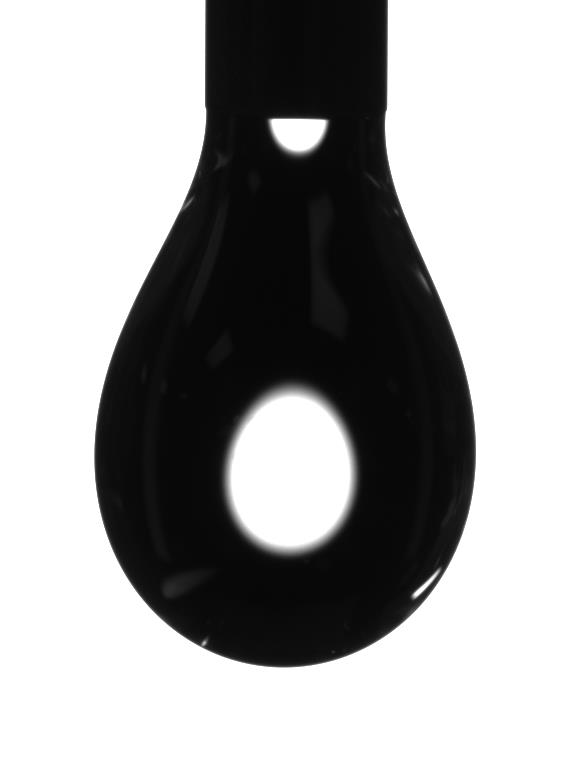
\includegraphics[width=0.5\linewidth]{pendant_drop.jpg}
  \caption{Висяща капка}
\end{minipage}%
\begin{minipage}{0.5\textwidth}
  \centering
  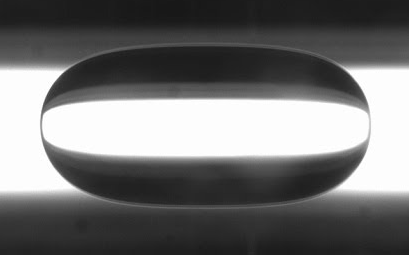
\includegraphics[width=0.6\linewidth]{index.png}
  \caption{Въртяща капка}
\end{minipage}
\end{figure}

\subsection{Задачата}
Задачата на проекта ни е да анализираме осевосиметрична капка на база профила ѝ. Понеже капката е осевосиметрична, е достатъчно да се наблюдава само една част от нейната повърхност. Цел на анализа е да се определят параметри, с помощта на които да може да се пресметне повърхностното напрежение на течността, от която се състои капката.

\section{Подход за определяне на формата на осевосиметрична капка}
    Методът ни на решаване на задачата има следните стъпки:
    \renewcommand{\labelenumi}{\roman{enumi}}
    \begin{enumerate}
        \item Извличане на експериментален профил на капка от входен файл или снимка;
        \item Генериране на теоретични профили;
        \item Пресмятане на грешката между теоретичен и експериментален профил;
        \item Определяне на теоретичния профил, който е най-близък до експерименталния профил (т.е. с най-малка грешка).
    \end{enumerate}

\section{Извличане на експериментален профил от снимка}
    Приемаме, че програмата ни е получила изображение на осевосиметрична капка, която виси от вертикална тръба. Заради симетричността ѝ е достатъчно да използваме само част от контура ѝ (т.е. червеното очертание на Фиг. 3), за да построим експерименталния ѝ профил т.е. как изглежда формата ѝ в експериментални условия.\\
\begin{figure}[H]
\centering
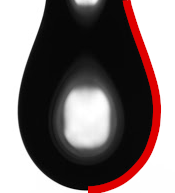
\includegraphics[width=0.2\linewidth]{pendant_drop_1_with_profile.png}
\caption{Профил на капката}
\end{figure}

Обработваме изображението със следния алгоритъм:
    
\renewcommand{\labelenumi}{\roman{enumi}}
\begin{enumerate}
    \item Изображението се замазва (чрез т.нар. Box blur).
    \item Цветовете на изображението се превръщат в сива гама.
    \item Намират се най-светлия и най-тъмния пиксел, чрез които се пресмята средния цвят на изображението.
    \item Изображението се обхожда ред по ред. Редът се обхожда докато се стигне до пиксел, който е по-тъмен от средния за изображението. Когато се стигне до такъв пиксел координатите му се добавят в масив от координати на точки и алгоритъма продължава с обхождането следващия ред (тъй като е достатъчна една точка от ред).
    \item Координатите се транслират, така че върхът да е в началото на координатната система и се скалират така, че най-горната точка да е на разстояние 1 от ординатата.
\end{enumerate}

Резултати от предложения по-горе алгоритъм за висящите капки на Фиг. 4 и Фиг. 6 са показани съответно на Фиг. 5 и Фиг. 7.

\begin{figure}[H]
\centering
\begin{minipage}{0.5\textwidth}
  \centering
  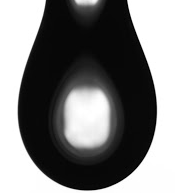
\includegraphics[width=0.5\linewidth]{pendant_drop_1.png}
  \caption{Първоначална снимка}
\end{minipage}%
\begin{minipage}{0.5\textwidth}
  \centering
  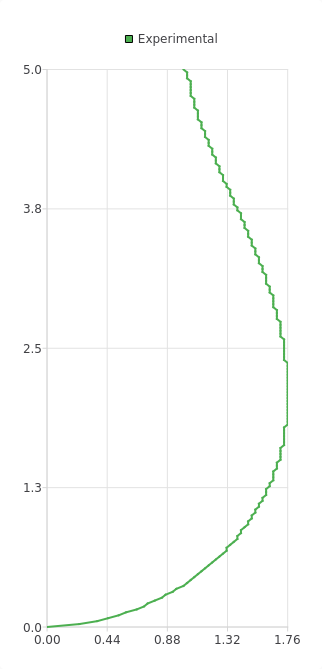
\includegraphics[width=0.4\linewidth]{pendant_drop_1_profile.png}
  \caption{Профил на капката}
\end{minipage}
\end{figure}
\begin{figure}[H]
\centering
\begin{minipage}{0.5\textwidth}
  \centering
  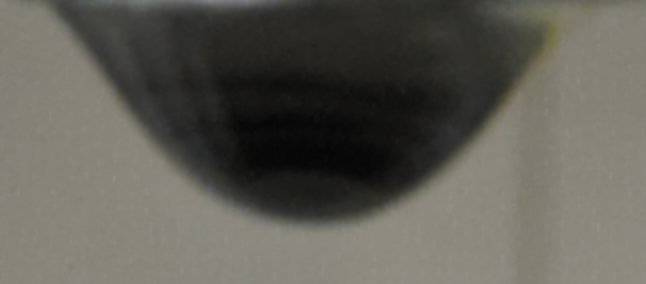
\includegraphics[width=0.5\linewidth]{pendant_real_deal_2.png}
  \caption{Първоначална снимка}
\end{minipage}%
\begin{minipage}{0.5\textwidth}
  \centering
  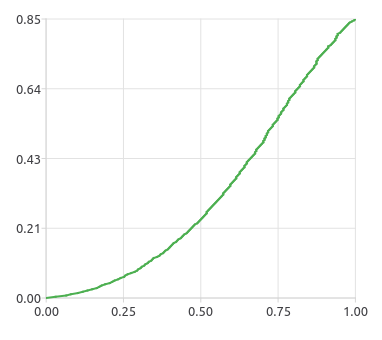
\includegraphics[width=0.6\linewidth]{l.png}
  \caption{Профил на капката}
\end{minipage}
\end{figure}
\section{Математически модел}
Теоретичният профил на капката представлява как тя би трябвало да изглежда спрямо дадени параметри. За да намерим теоретичен профил на капка, трябва да решим математическия модел. Той се извежда с помощта на уравнението на Юнг-Лаплас и геометричните свойства на капката.
\subsection{Уравнение на Юнг-Лаплас}
\normalsize
Уравнението на Юнг-Лаплас е нелинейно частно дифериенциално уравнение, което описва зависимостта между напрежението в дадена капка, кривината ѝ, и нейното повърхностно напрежение.\\
Уравнението изглежда така:
\begin{center}
$\Delta \rho = \sigma ( \frac {1}{R_1} + \frac {1}{R_2}) $,
\end{center}
като $\Delta \rho$ е разликата между наляганията в капката и извън нея,
${R_1}$ и ${R_2}$ са главните кривини на капката, а $\sigma$ е повърхностното напрежение на течността на капката.

\subsection{Извеждане на математическия модел}
От \cite{ASDA_report} имаме следната система диференциални уравнения:
\begin{align*}
\frac {dx}{ds} &= \cos \varphi\\
\frac {dz}{ds} &= \sin \varphi\\
\frac {d\varphi}{ds} &= \frac{\Delta p}{\sigma} - \frac{\sin \varphi}{x},
\end{align*}
където първите две уравнения идват от геометрични съображения за формата на капката, а третото е уравнението на Юнг-Лаплас. С \(x\) и \(z\) са означени координатите на всяка точка от профила на капката, \(\varphi\) е ъгъла между допирателната през дадена точка от профила и абсцисната ос, а \(ds\) е дължината на дъгата между две близки точки от профила на капката.\\

Понеже $\Delta p = \Delta p_0 + \Delta \rho gz$, където $\Delta p_0$ е налягането на върха на капката, можем да приложим още веднъж уравнението на Юнг-Лаплас и като означим кривината на върха на капката с $R_0$ получаваме: $p_0 = \frac{2\sigma}{R_0}$\\
След заместване в предната система получаваме:
\begin{align*}
\frac {dx}{ds} &= \cos \varphi\\
\frac {dz}{ds} &= \sin \varphi\\
\frac {d\varphi}{ds} &= \frac {2} {R_0}  + \frac{\Delta \rho gz}{\sigma} - \frac{\sin \varphi}{x}
\end{align*}

Въвеждаме означенията
\large
\(b\!:=\frac{1}{R_0}\) \normalsize и \large \(c\!:=\frac{\Delta \rho g}{\sigma}\) 
\normalsize и получаваме следната система диференциални уравнения, зависеща от коефициентите \(b\) и \(c\):
\begin{align}
\begin{split} 
\frac {dx}{ds} &= \cos \varphi\label{simul1}\\
\frac {dz}{ds} &= \sin \varphi\\
\frac {d\varphi}{ds} &= 2b + cz - \frac{\sin \varphi}{x}
\end{split}
\end{align}
Понеже системата не е дефинирана във върха на капката, за начални условия използваме \(x(0)=0\), \(z(0)=0\), \(\varphi(0)=0\). При третото уравнение имаме проблем, когато \(s=0\), но по дефиниция имаме, че при \(s=0\) (т.е. във върха на капката), \large\begin{math}{\frac{d\varphi}{ds} = b}\end{math}\normalsize.\\
За въртяща капка получаваме подобна система:
\begin{align}
\begin{split}
\frac {dx}{ds} &= \cos \varphi\label{simul2}\\
\frac {dz}{ds} &= \sin \varphi\\
\frac {d\varphi}{ds} &= 2b + dx^2 - \frac{\sin \varphi}{x}
\end{split}
\end{align}
където 
\large
\(b\!:=\frac{1}{R_0}\) \normalsize и \large \(d\!:=\frac{\omega}{2\sigma}\). 
\normalsizeПри решаването на модела за въртяща капка, използваме същите начални стойности като при висяща капка.\\
От тук нататък ще се занимаваме само с висящи капки, като разглеждаме системата \eqref{simul1}, заедно с началните условия.

\section{Решаване на математическия модел}
Ако разполагаме със стойности на параметрите b и c, то решението на системата от диференциални уравнения \eqref{simul1} и \eqref{simul2} (с посочените по-горе начални условия), ще бъде теоретичния профил на капка с тези параметри. За целта използваме метода на Рунге-Кута от четвърти ред \cite{runge-kutta}. Това е итеративен метод за приближено решаване на задачата на Коши.\\
Нека например разгледаме:
\begin{align*}
    \frac{dy}{dx} &= f(x, y), x \in {(0,x]}\\
    y(0) &= y_0
\end{align*}
То методът на Рунге-Кута от четвърти ред изглежда така:
\begin{align*}
    k_1 &= hf(x_n, y_n)\\
    k_2 &= hf(x_n + \frac{h}{2}, y_n + \frac{k_1}{2})\\
    k_3 &= hf(x_n + \frac{h}{2}, y_n + \frac{k_2}{2})\\
    k_4 &= hf(x_n + h, y_n + k_3)\\
    y_{n+1} &= y_n + k_1/6 + k_2/3 + k_3/3 + k_4/6
\end{align*}
Като приложим този метод за висящи капки, получаваме:
\begin{align*}
    (x_0, z_0, \varphi_0) &= (0, 0, 0)\\
    f(x, z, \varphi) &= \left\{\begin{array}{lr}(\cos \varphi, \quad \sin \varphi, \quad 2b + cz - \sin(\varphi) / n), &\textup{ако } x \neq 0,\\(\cos \varphi, \quad \sin \varphi, \quad b), &\textup{ако } x = 0 \end{array}\right\}\\
    (k_{1,n}, l_{1,n}, m_{1,n}) &= hf(x_n, \quad z_n, \quad \varphi_n)\\
    (k_{2,n}, l_{2,n}, m_{2,n}) &= hf(x_n + \frac{k_{1,n}}{2}, \quad z_n + \frac{l_{1,n}}{2}, \quad \varphi_n + \frac{m_{1,n}}{2})\\
    (k_{3,n}, l_{3,n}, m_{3,n}) &= hf(x_n + \frac{k_{2,n}}{2}, \quad z_n + \frac{l_{2,n}}{2}, \quad \varphi_n + \frac{m_{2,n}}{2})\\
    (k_{4,n}, l_{4,n}, m_{4,n}) &= hf(x_n + k_{3,n}, \quad z_n + l_{3,n}, \quad \varphi_n + m_{3,n})\\
    \begin{bmatrix} x_{n+1} \\ z_{n+1} \\ \varphi_{n+1} \end{bmatrix} &= \begin{bmatrix} x_n \\ z_n \\ \varphi_n \end{bmatrix} + \frac{1}{6} \left( \begin{bmatrix} k_{1,n} \\ l_{1,n} \\ m_{1,n} \end{bmatrix} + 2\begin{bmatrix} k_{2,n} \\ l_{2,n} \\ m_{2,n} \end{bmatrix} + 2\begin{bmatrix} k_{3,n} \\ l_{3,n} \\ m_{3,n} \end{bmatrix} + \begin{bmatrix} k_{4,n} \\ l_{4,n} \\ m_{4,n} \end{bmatrix}\right)
\end{align*}

Решаваме задачата, докато $x_n <= 1$.

Резултати от метода се показани на Фиг. 8 и Фиг. 9, където в син цвят е начертан получен чрез метода профил, а със зелено - експериментално получен профил с вече известни параметри. Наблюдава се, че дори и при относително голяма стъпка ($h = 0.1$) полученият профил е много близък до експерименталния, стига да му бъдат подадени достатъчно точни стойности за \(b\) и \(c\).

\begin{figure}[H]
\centering
\begin{minipage}{0.5\textwidth}
  \centering
  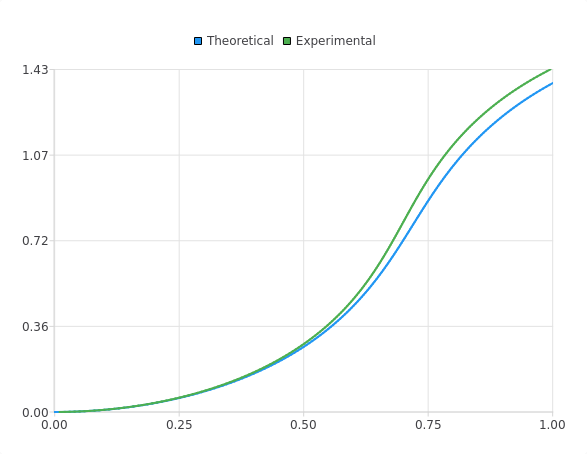
\includegraphics[width=1\linewidth]{app-theoretical-1.png}
  \caption{Генериране на теоретичен профил \protect\\ Експериментални: b = 1.843658, c = -2.9 \protect\\ Входни: b = 1.8, c = -2.9 при h = 0.1}
\end{minipage}%
\begin{minipage}{0.5\textwidth}
  \centering
  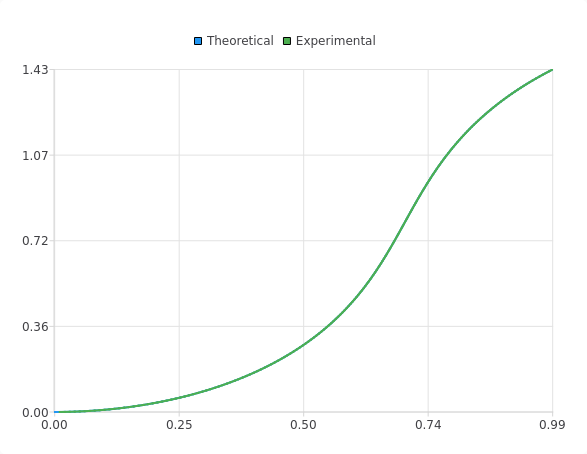
\includegraphics[width=1\linewidth]{app-theoretical-2.png}
  \caption{Генериране на теоретичен профил \protect\\ Експериментални: b = 1.843658, c = -2.9 \protect\\ Входни: b = 1.843658, c = -2.9 при h = 0.1}
\end{minipage}
\end{figure}

\section{Намиране на грешка между теоретичен и експериментален профил}
При дадени теоретичен и експериментален профили на капки ще ни бъде необходимо да намерим разликата между тези два профила, т.е. грешката на теоретичния профил спрямо експерименталния. Търсеният алгоритъм е необходимо да отговаря на следните изисквания:
\begin{itemize}
    \item Да може да бъде приложим върху два случайни профила, тоест да работи, когато:
    \begin{itemize}
        \item единият профил е по-голям от другия, например ако x/y координатите на единия профил са в интервала [0,1], но тези на другия профил са в интервала [0, 5];
        \item профилите не могат да бъдат представени като функции на една променлива, тоест профилите могат да имат две или повече точки с еднакви стойности на x и/или y координатите.
    \end{itemize}
    \item Да има кратко време за изпълнение.
\end{itemize}
За намиране на грешката е приложен следният алгоритъм:
\renewcommand{\labelenumi}{\arabic{enumi}}
\begin{enumerate}
    \item За всяка точка от двата профила се намира разстоянието от нея до върха на профила. Това разстояние се изчислява като сума от разстоянията между всеки две съседни точки, намиращи се между въпросната точка и върха на профила:
    \begin{algorithm}[H]
        profile = масив от точките на даден профил\;
        $profile[1].value = 0$\;
        \For{$i \in \{2, 3, ..., length(profile)\}$}{
            $x = profile[i].x - profile[i - 1].x$\;
            $y = profile[i].y - profile[i - 1].y$\;
            $dist = \sqrt{x^2 + y^2}$\;
            $profile[i].value = profile[i - 1].value + dist$\;
        }
    \end{algorithm}
    \newpage
    \item Стойностите на точките в двата профила се ''нормализират'', тоест всички стойности се разделят на максималната стойност в профила. След това стойностите на всички точки от профила ще бъдат в интервала [0,1];
    \begin{algorithm}[H]
        $m = max(profile.value)$\;
        \For{$point \in profile$}{
            $point.value = point.value / m$\;
        }
    \end{algorithm}
    \item За всяка точка \(p1\) от експерименталния профил се намира точката \(p2\) от теоретичния профил, чиято стойност е възможно най-близка до тази на точката \(p1\). Изчислява се разстоянието между тези две точки;
    \item За стойност на грешката между двата профила се взема сумата от квадратите на намерените в точка 3 разстояния.
    \begin{algorithm}[H]
        $error = 0$\;
        $t = 1$\;
        \For{$p1 \in experimental$}{
            \While{$t < length(theoretical) \quad or \quad |theoretical[t].value - p1.value| > |theoretical[t + 1].value - p1.value|$}{
                $t = t + 1$\;
            }
            $p2 = theoretical[t]$\;
            $x = p1.x - p2.x$\;
            $y = p1.y - p2.y$\;
            $error = error + (x^2 + y^2)$\;
        }
    \end{algorithm}

\end{enumerate}
Представеният алгоритъм е осъществен със сложност O(N + M), където N и M са съответно броя на точките в първия и втория профил.

\section{Намиране на най-близък теоретичен профил}
За да намерим теоретичен профил, който е възможно най-близък до експерименталния профил, използваме методът на най-бързото спускане така че при зададени начални стойности на \(b\) и \(c\), да се намери стойност на \(c\), при която грешката е минимална. За да се проверяват различни стойности на \(b\) и да се избегне погрешното намиране на локален вместо глобален минимум, използваме таблица от различни начални стойности на $b$ и $c$. Текущата итерация на програмата използва следните начални стойности:

\begin{align*}
\begin{split} 
B &= \{0.1 + \frac{2.9i}{100} | i = 0, 1, 2, ..., 100\}\\
C &= \{-6 + \frac{6i}{15} | i = 0, 1, 2, ..., 15\}\\
\end{split}
\end{align*}
$$(b,c) \in B \times C $$

На Фиг.10 и Фиг.11 са показани намерените най-близки теоретични профили за висяща капка с известни експериментални данни, като графиката в зелено е експерименталният профил, а тази в синьо - теоретичният. И двата резултата са получени след изпълняване на алгоритъма за минимизиране на грешката. Разликата между Фиг. 10 и Фиг. 11 е стъпката, с която е изпълнен споменатият алгоритъм (съответно 0.1 и 0.01). Колкото по-малка е стъпката \(h\), толкова по-точен теоретичен профил получаваме (може да се види, че на Фиг. 11 двете графики почти съвпадат).

\begin{figure}[H]
\centering
\begin{minipage}{0.5\textwidth}
  \centering
  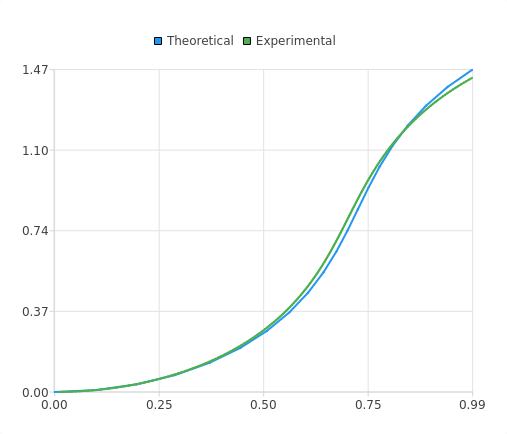
\includegraphics[width=1\linewidth]{gradient-descent-1-0.1.png}
  \caption{Минимизиране на грешката (висяща) \protect\\ Експериментални: b = 1.843658, c = -2.9 \protect\\ Изходни: b = 1.782, c = -2.66419635 при h = 0.1}
\end{minipage}%
\begin{minipage}{0.5\textwidth}
  \centering
  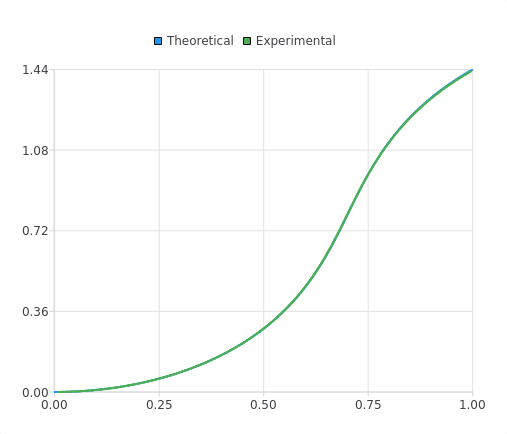
\includegraphics[width=1\linewidth]{gradient-descent-1-0.01.png}
  \caption{Минимизиране на грешката (висяща) \protect\\ Експериментални: b = 1.843658, c = -2.9 \protect\\ Изходни: b = 1.84, c = -2.88179338 при h = 0.01}
\end{minipage}
\end{figure}

На Фиг. 12 и Фиг. 13 са показани получените теоретични профили за съответните въртящи капки, входните данни за които са ни известни. Зелената графика е експерименталният профил, а синята - теоретичният. Разликата между двете фигури е отново стъпката \(h\) и се наблюдава, че с по-малка стъпка, получаваме по-точен теоретичен профил

\begin{figure}[H]
\centering
\begin{minipage}{0.5\textwidth}
  \centering
  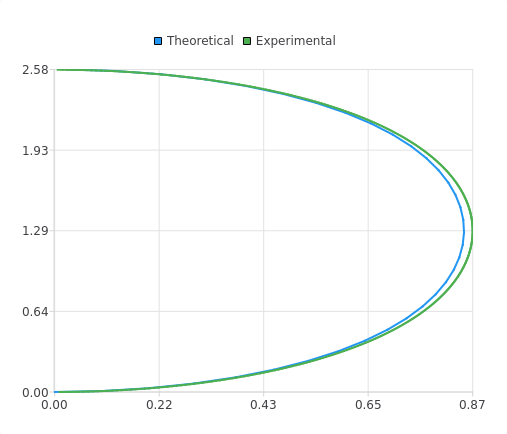
\includegraphics[width=1\linewidth]{gradient-descent-2-0.1.png}
  \caption{Минимизиране на грешката (въртяща) \protect\\ Експериментални: b = 1.504438, c = -1.873 \protect\\ Изходни: b = 1.55, c = -2.07054505 при h = 0.1}
\end{minipage}%
\begin{minipage}{0.5\textwidth}
  \centering
  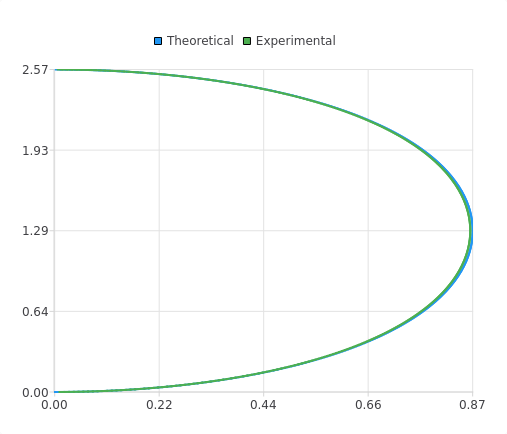
\includegraphics[width=1\linewidth]{gradient-descent-2-0.01.png}
  \caption{Минимизиране на грешката (въртяща) \protect\\ Експериментални: b = 1.504438, c = -1.873 \protect\\ Изходни: b = 1.492, c = -1.82101084 при h = 0.01}
\end{minipage}
\end{figure}


\section{Имплементация на приложението}

Приложението е разрабонето с езика C++ и библиотеката Qt. За неговия интерфейс използваме Qt библиотеката ''Qt Quick Controls 2'', която му позволява да бъде използван на много различни платформи, включително Windows, Linux и Android. За изчертаване на графиките използваме ''Qt Charts''. Използвани са версии Qt5.14 и C++17.
Приложението позволява зареждане на експериментален профил от текстови файл, изображение, запазено на устройството и също така предоставя опцията да се направи снимка на капка от самото приложение. При натискане на бутона ''Minimize theoretical error'' паралелно се изпълнява метода на най-бързото спускане с множество различни начални точки и резултатът от това изпълнение се показва на екрана.
Кодът на приложението може да бъде намерен на \texttt{\url{https://github.com/pgeorgiev98/drop_shape_analysis} }\\
\newline
\hspace*{3ex}На Фиг. 14 и Фиг. 15 са показани изгледи от интерфейса на приложението, съответно теоретичен и експериментален профил за висяща капка със стъпка \(h = 0.01 \) на Фиг. 14 и графика на грешката между тях на Фиг. 15. Фигури 16, 17 и 18 показват резултати на програмата за различни висящи капки.

\begin{figure}[H]
\centering
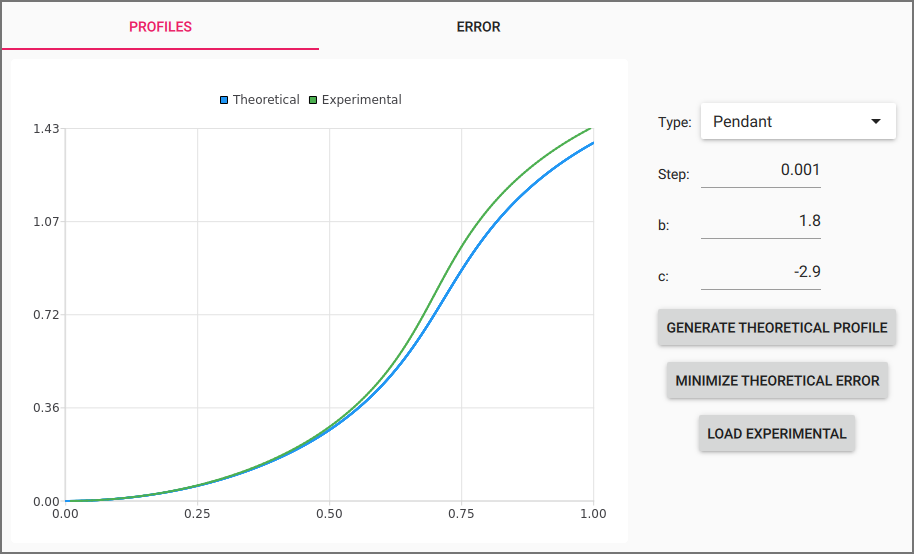
\includegraphics[width=0.8\textwidth]{app-1.png}
\caption{Изглед от приложението}
\end{figure}

\begin{figure}[H]
\centering
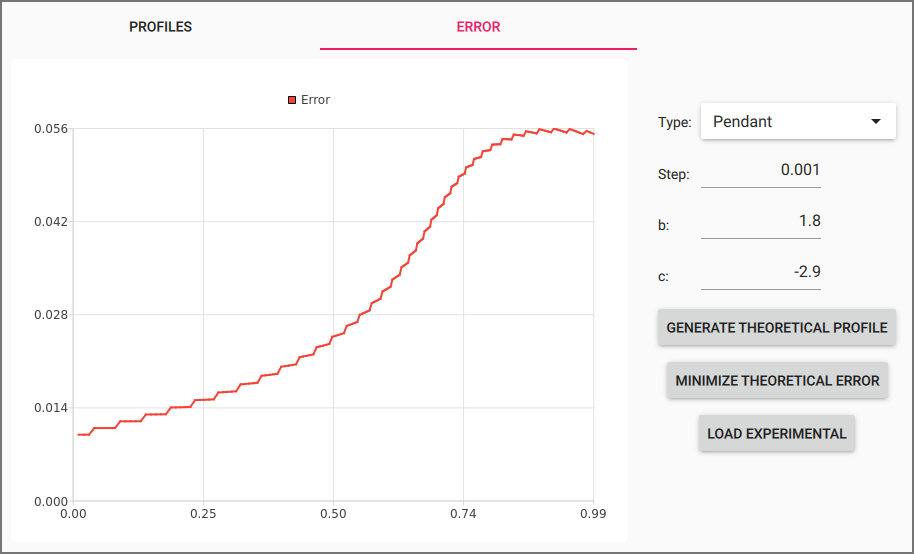
\includegraphics[width=0.8\textwidth]{app-2.png}
\caption{Изглед от приложението}
\end{figure}

\begin{figure}[H]
\centering
\begin{minipage}{0.5\textwidth}
  \centering
  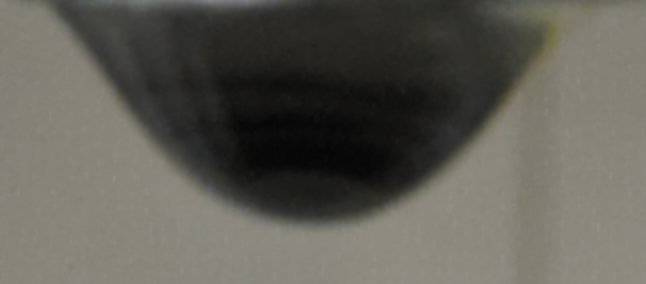
\includegraphics[width=0.9\linewidth]{pendant_real_deal_2.png}
\end{minipage}%
\begin{minipage}{0.5\textwidth}
  \centering
  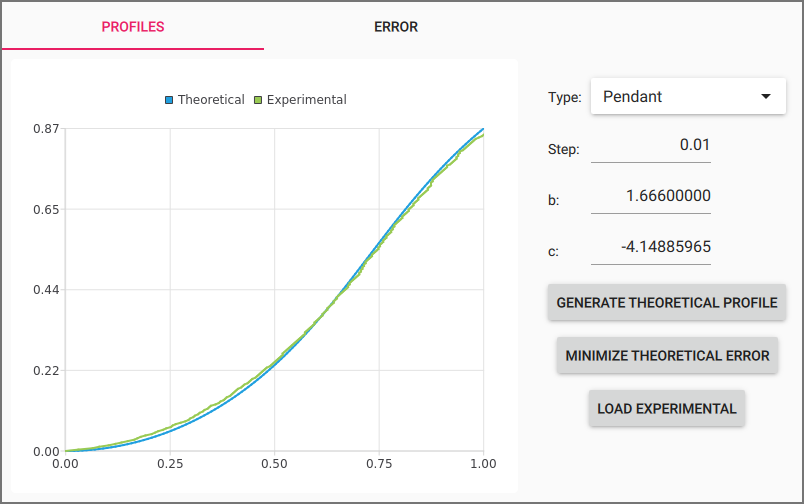
\includegraphics[width=0.9\linewidth]{app_real_deal_2.png}
\end{minipage}
\caption{Резултати от приложението при снимка на висяща капка}
\end{figure}

\begin{figure}[H]
\centering
\begin{minipage}{0.5\textwidth}
  \centering
  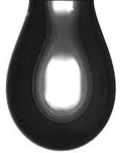
\includegraphics[width=0.45\linewidth]{pendant_drop_4.png}
\end{minipage}%
\begin{minipage}{0.5\textwidth}
  \centering
  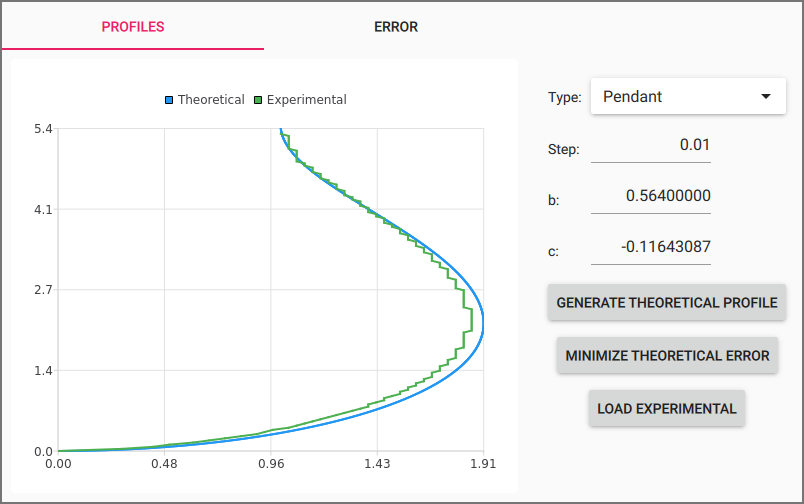
\includegraphics[width=0.9\linewidth]{app_pendant_4.png}
\end{minipage}
\caption{Резултати от приложението при снимка на висяща капка}
\end{figure}

\begin{figure}[H]
\centering
\begin{minipage}{0.5\textwidth}
  \centering
  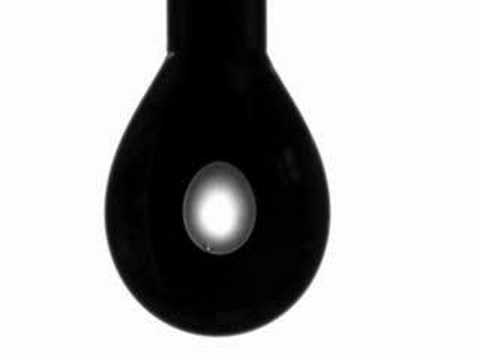
\includegraphics[width=0.7\linewidth]{new_pendant_1.jpg}
\end{minipage}%
\begin{minipage}{0.5\textwidth}
  \centering
  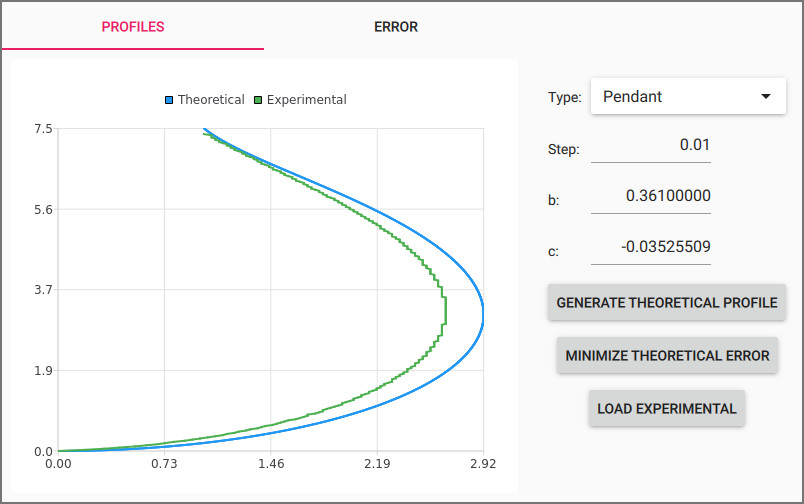
\includegraphics[width=0.9\linewidth]{app_new_pendant_1.jpg}
\end{minipage}
\caption{Резултати от приложението при снимка на висяща капка}
\end{figure}
\section{Заключение}
Занимавахме се с това да намерим приближена стойност на повърхностното напрежение на течност, като намираме коефициенти, от които зависи формата на капка от течността.\\
Методът на Рунге-Кута предоставя достатъчно точно решение на математическия модел за малък брой итерации. Предложеният алгоритъм за намиране на грешката предоставя задоволителни резултати за линейно време. Това ни ползволява да изпълняваме метода на най-бързото спускане за голям брой начални параметри с малка стъпка при решаването на модела. Всичко това прави възможно бързото намиране на теоретичен профил, близък до даден експериментален.
\newpage

\begin{thebibliography}{9}
\bibitem{ASDA_report} 
Galina Lyutskanova, Kiril Mihaylov, Vasil Kolev.
\textit{Axisymmetric Drop Shape Analysis}. 
Faculty of Mathematics and Informatics, Sofia University, 2015.

\bibitem{surfsource} 
R. Nave, \textit{Surface Tension}
\\\texttt{\url{http://hyperphysics.phy-astr.gsu.edu/hbase/surten.html}}

\bibitem{runge-kutta}
\texttt{\url{https://math.stackexchange.com/q/721076}}

\end{thebibliography}

\end{document}
